\documentclass{article}

\usepackage{enumitem}
\usepackage{listings}
\usepackage{graphicx}
\usepackage{float}

\usepackage{color} %red, green, blue, yellow, cyan, magenta, black, white
\definecolor{mygreen}{RGB}{28,172,0} % color values Red, Green, Blue
\definecolor{mylilas}{RGB}{170,55,241}
\usepackage{float}
\usepackage{hyperref}

\title{CS5487 Programming Assignment 1}
\date{2019 October}
\author{Ji Yang}

\begin{document}
\maketitle

\lstset{language=Matlab,%
    %basicstyle=\color{red},
    breaklines=true,%
    morekeywords={matlab2tikz},
    keywordstyle=\color{blue},%
    morekeywords=[2]{1}, keywordstyle=[2]{\color{black}},
    identifierstyle=\color{black},%
    stringstyle=\color{mylilas},
    commentstyle=\color{mygreen},%
    showstringspaces=false,%without this there will be a symbol in the places where there is a space
    numbers=left,%
    numberstyle={\tiny \color{black}},% size of the numbers
    numbersep=9pt, % this defines how far the numbers are from the text
    emph=[1]{for,end,break},emphstyle=[1]\color{red}, %some words to emphasise
    %emph=[2]{word1,word2}, emphstyle=[2]{style},    
}

\section*{Polynomial Function}
\subsection*{(a) Implement 5 regression algorithms}
Source code can be found at \url{https://github.com/yangji12138/machine-learning/tree/master/Programming%201} or the Codes Appendix.

\subsection*{(b) Using Sample Data to estimate 5-th order poly function}

\begin{table}[H]
    \begin{tabular}{|c|c|c|c}
    \hline
        & Least-Sqaures (LS)     & \begin{tabular}[c]{@{}c@{}}Regularized LS (RLS)\\ $\lambda$ = 0.48\end{tabular} & \multicolumn{1}{c|}{\begin{tabular}[c]{@{}c@{}}L1-Regularized LS (LASSO)\\ $\lambda$ = 0.48\end{tabular}} \\ \hline
    MSE & 0.4086                 & 0.4076                                                                       & \multicolumn{1}{c|}{0.4086}                                                                            \\ \hline
        & Robust Regression (RR) & Bayesian Regression (BR)                                                     &                                                                                                        \\ \cline{1-3}
    MSE & 0.7680                 & 0.4592                                                                       &                                                                                                        \\ \cline{1-3}
    \end{tabular}
\end{table}

\begin{figure}[H]
    \centering
    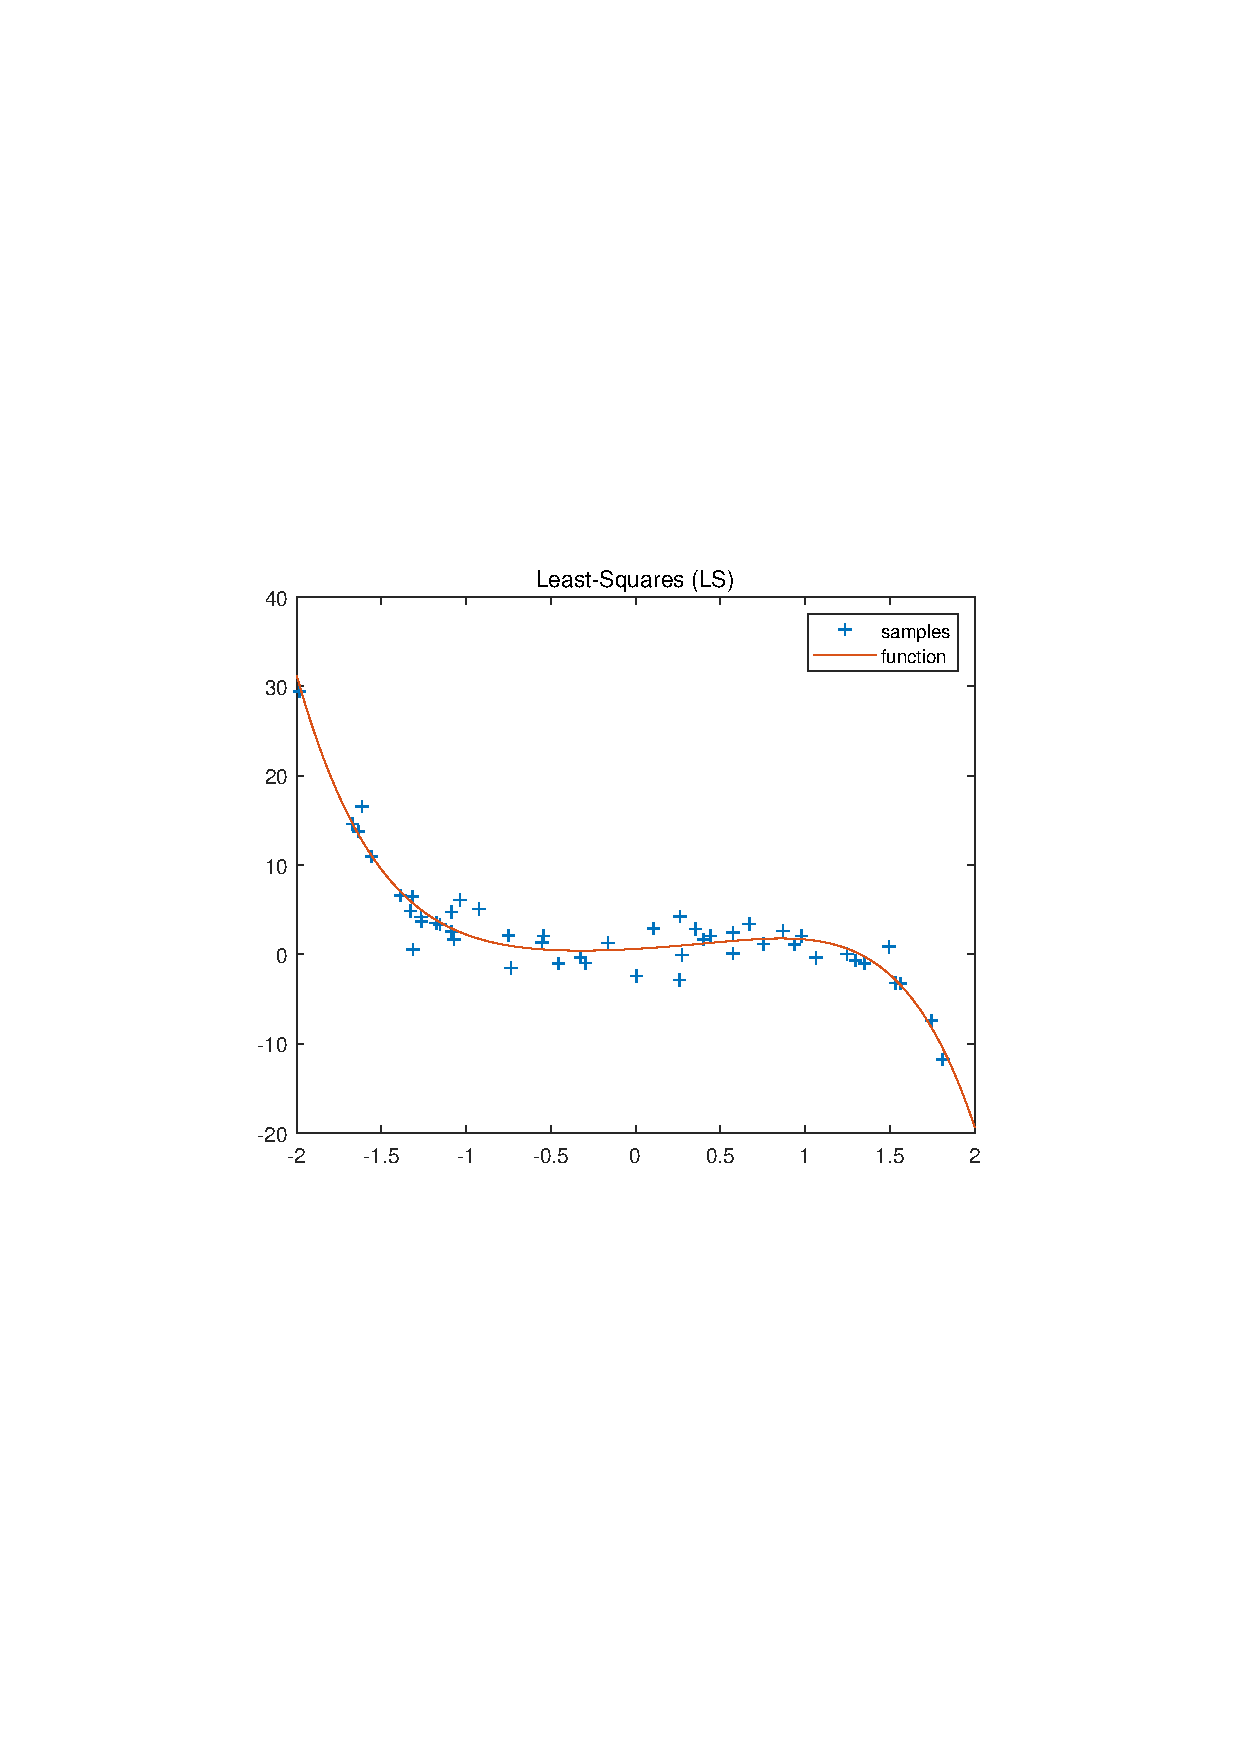
\includegraphics[width=\textwidth]{fig/1b-ls.pdf}
    \label{fig:1b-ls}
\end{figure}


\subsection*{Conclusion}
Observe the experiment results, we can find that:

\begin{enumerate}[label=(\roman*)]
    \item For London, the cells could be approximately divided into two clusters: 45\%($\pi$) 0.8($\lambda$); 55\%($\pi$) 1.0($\lambda$).
    \item For Antwerp, the cells could be approximately divided into two clusters: 40\%($\pi$) 0.85($\lambda$); 60\%($\pi$) 2.3($\lambda$).
\end{enumerate}

\subsection*{Codes}

Source code can be found at \url{https://github.com/yangji12138/machine-learning/tree/master/Programming%201}.

%\lstinputlisting{../costFunction.m}



\end{document}